% !TEX root = ../main.tex
\section{Identificación de vegetación saludable y tipos de cultivo}

    % Recuadro de color para identificar los grupos de k-medias en la tabla
    \newcommand{\grupo}[2]{\textcolor[HTML]{#1}{\rule{0.8em}{0.8em}}~\textbf{#2}}

    Se trabajó con la escena del 03/04/2024 (Landsat 9, órbita 224/079, sin nubes), convertida a reflectancia de superficie igual que en la actividad anterior \cite{ej2_usgs_l2}. Las bandas de interés son la 3 (verde), la 5 (infrarrojo cercano, NIR) y la 6 (infrarrojo de onda corta 1, SWIR~1). La elección de bandas, su orden en la composición y la mejora de contraste se comprobaron con mediciones sobre la imagen, y la composición elegida se aplicó después a la escena completa.

    \subsection{Zonas y áreas de muestra}

        Se eligieron tres zonas de 30~km de lado ($1000 \times 1000$ píxeles) con paisajes distintos (\textbf{Figuras \ref{fig:ej3_escena} y \ref{fig:ej3_zonas}}):

        \begin{itemize}
            \item \textbf{Zona A:} agricultura mecanizada de Itapúa (Paraguay), para estudiar los tipos y estados de cultivo.
            \item \textbf{Zona B:} alrededores de Apóstoles, con yerbales, forestaciones, pastizales y monte.
            \item \textbf{Zona C:} selva paranaense continua sobre la Sierra Central de Misiones, la vegetación más densa de la escena.
        \end{itemize}

        Además se marcaron, por fotointerpretación, áreas de muestra de cada cobertura: rectángulos de 0,2 a 1,4~km$^2$ sobre una sola cobertura, para medir su respuesta sin mezclas. Una misma cobertura puede variar mucho de un lugar a otro, por eso las que más varían llevan más muestras. La selva tiene cuatro áreas, tres de ellas en la sierra, con laderas al sol y en sombra, y el pinar tiene cuatro plantaciones distintas, reconocibles por sus bloques rectangulares con cortafuegos, cada área dentro de un solo compartimento (\textbf{Figura \ref{fig:ej3_muestras}}). Los estados de cultivo se muestrearon con uno a tres lotes. Las mismas áreas se usaron para todas las mediciones y para entrenar la clasificación.

        \begin{figure}[H] \centering
            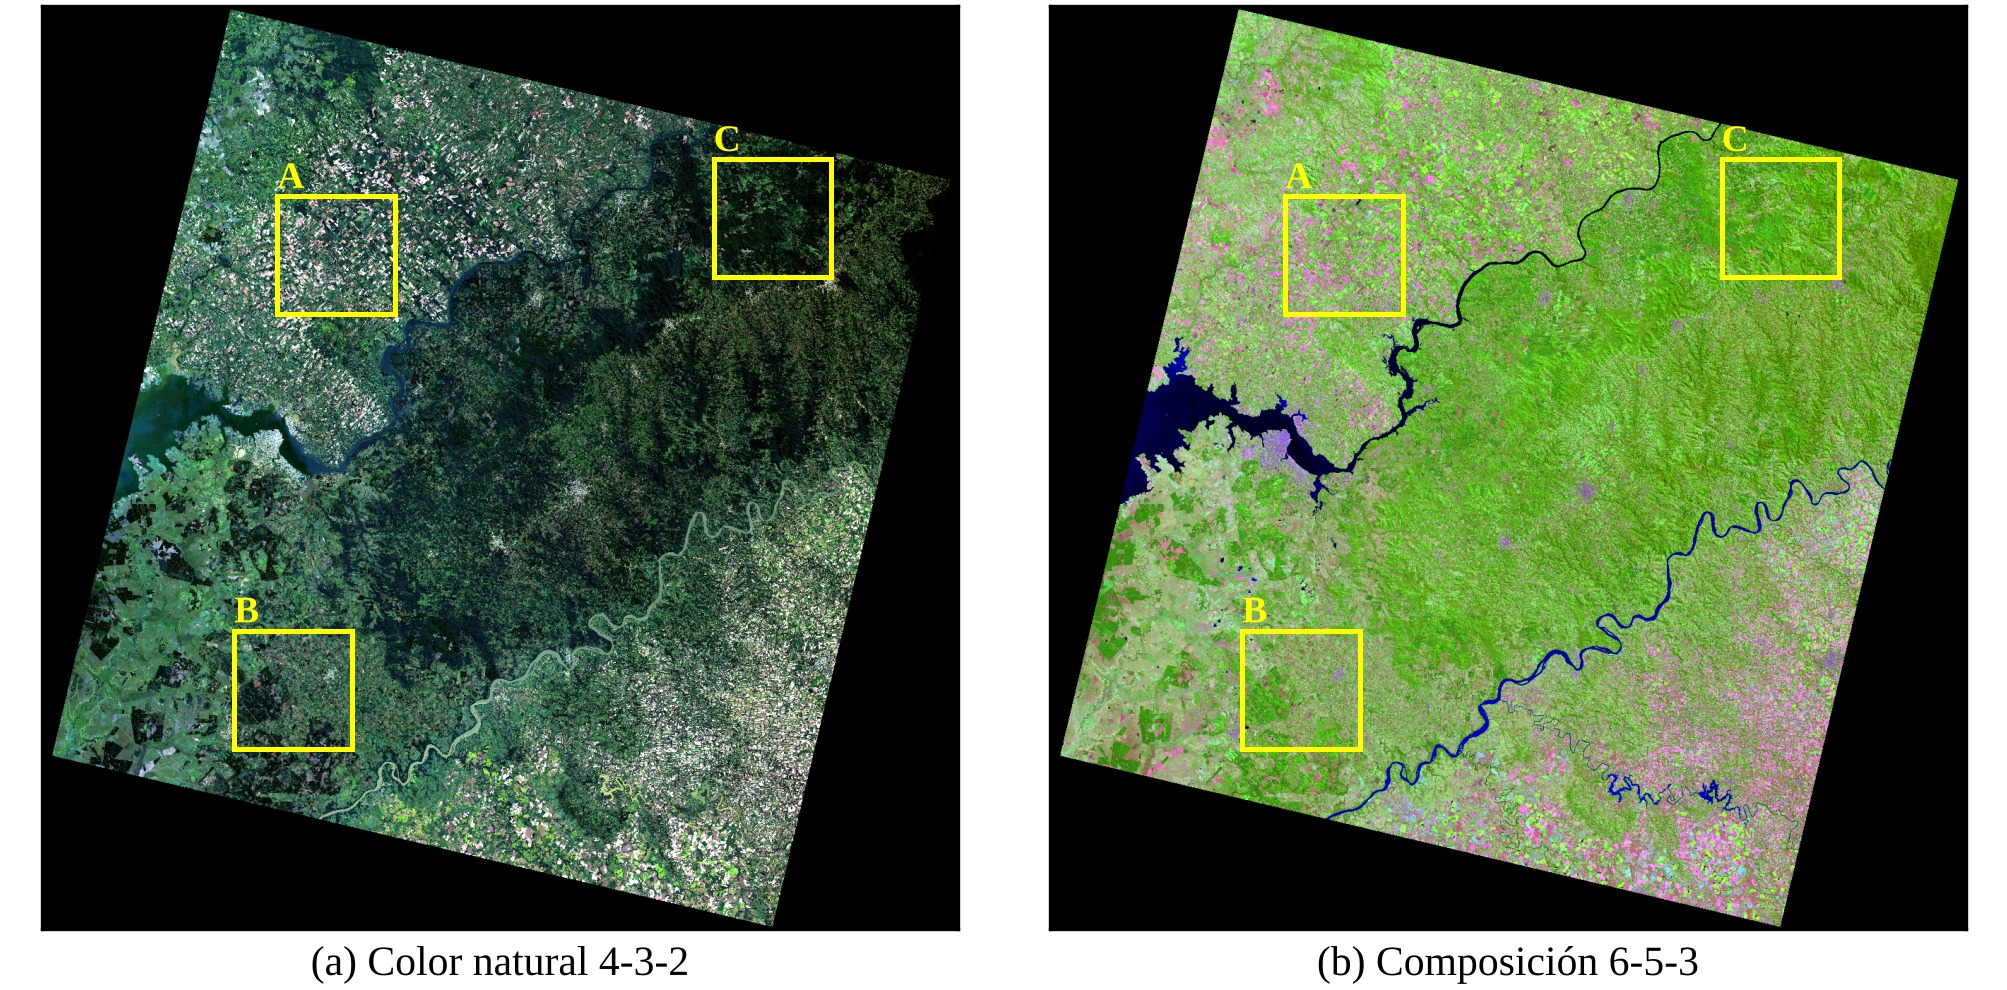
\includegraphics[width=.55\linewidth]{img/ejercicio3/escena.jpg}
            \caption{Zonas A, B y C sobre la escena completa.}
            \label{fig:ej3_escena}
        \end{figure}

        \begin{figure}[H] \centering
            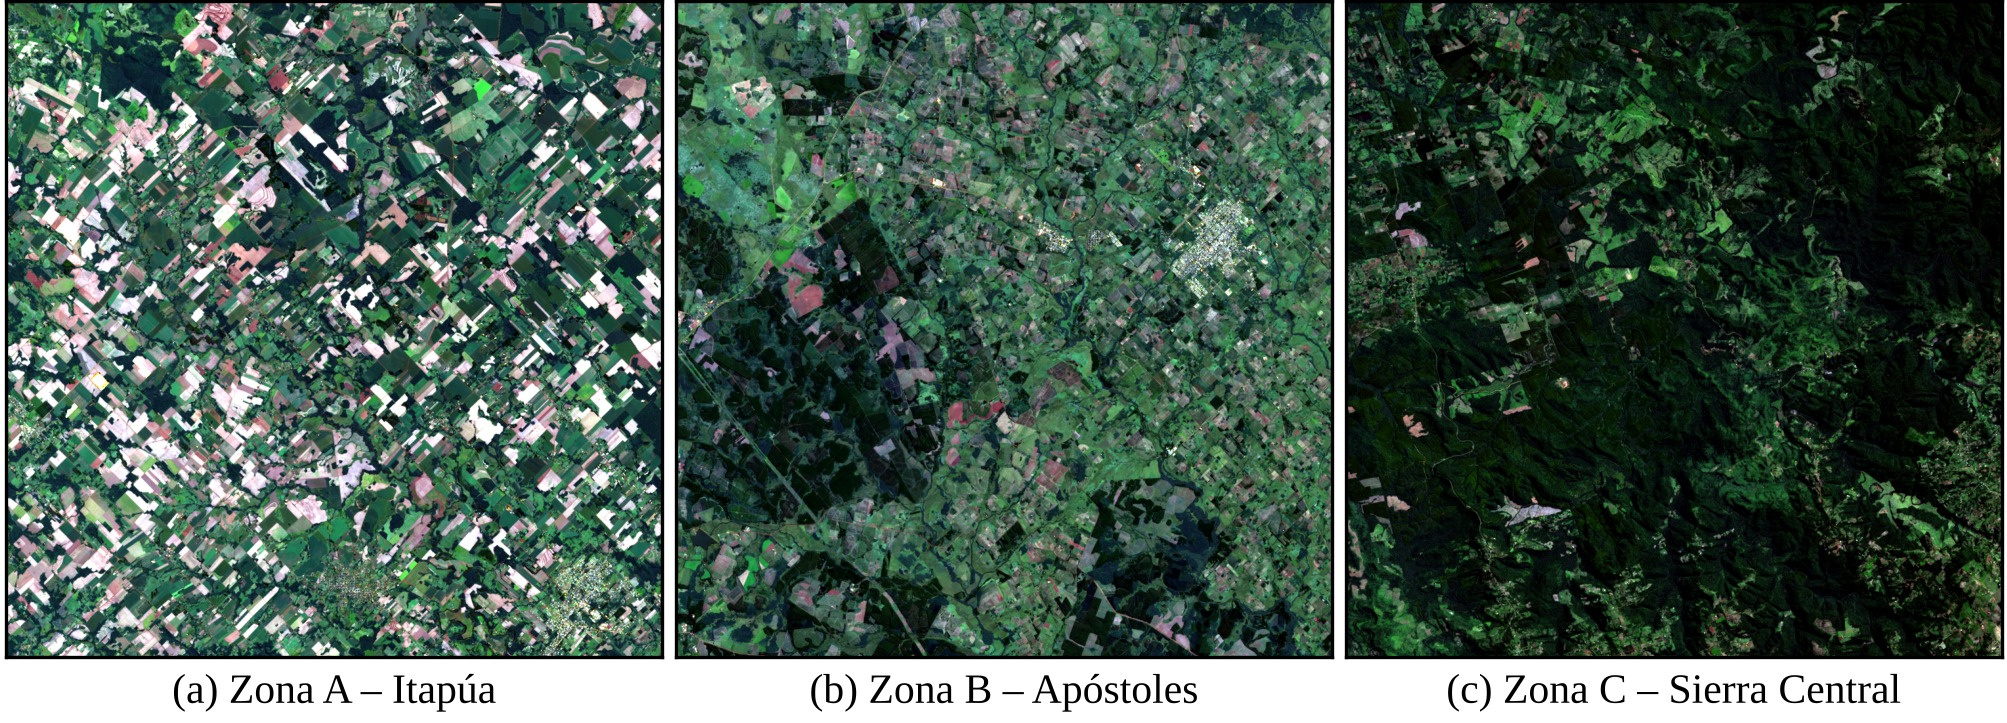
\includegraphics[width=\linewidth]{img/ejercicio3/zonas_rgb.jpg}
            \caption{Zonas de estudio en color natural (4-3-2), a resolución completa (30~m por píxel, 30~km de lado).}
            \label{fig:ej3_zonas}
        \end{figure}

        \begin{figure}[H] \centering
            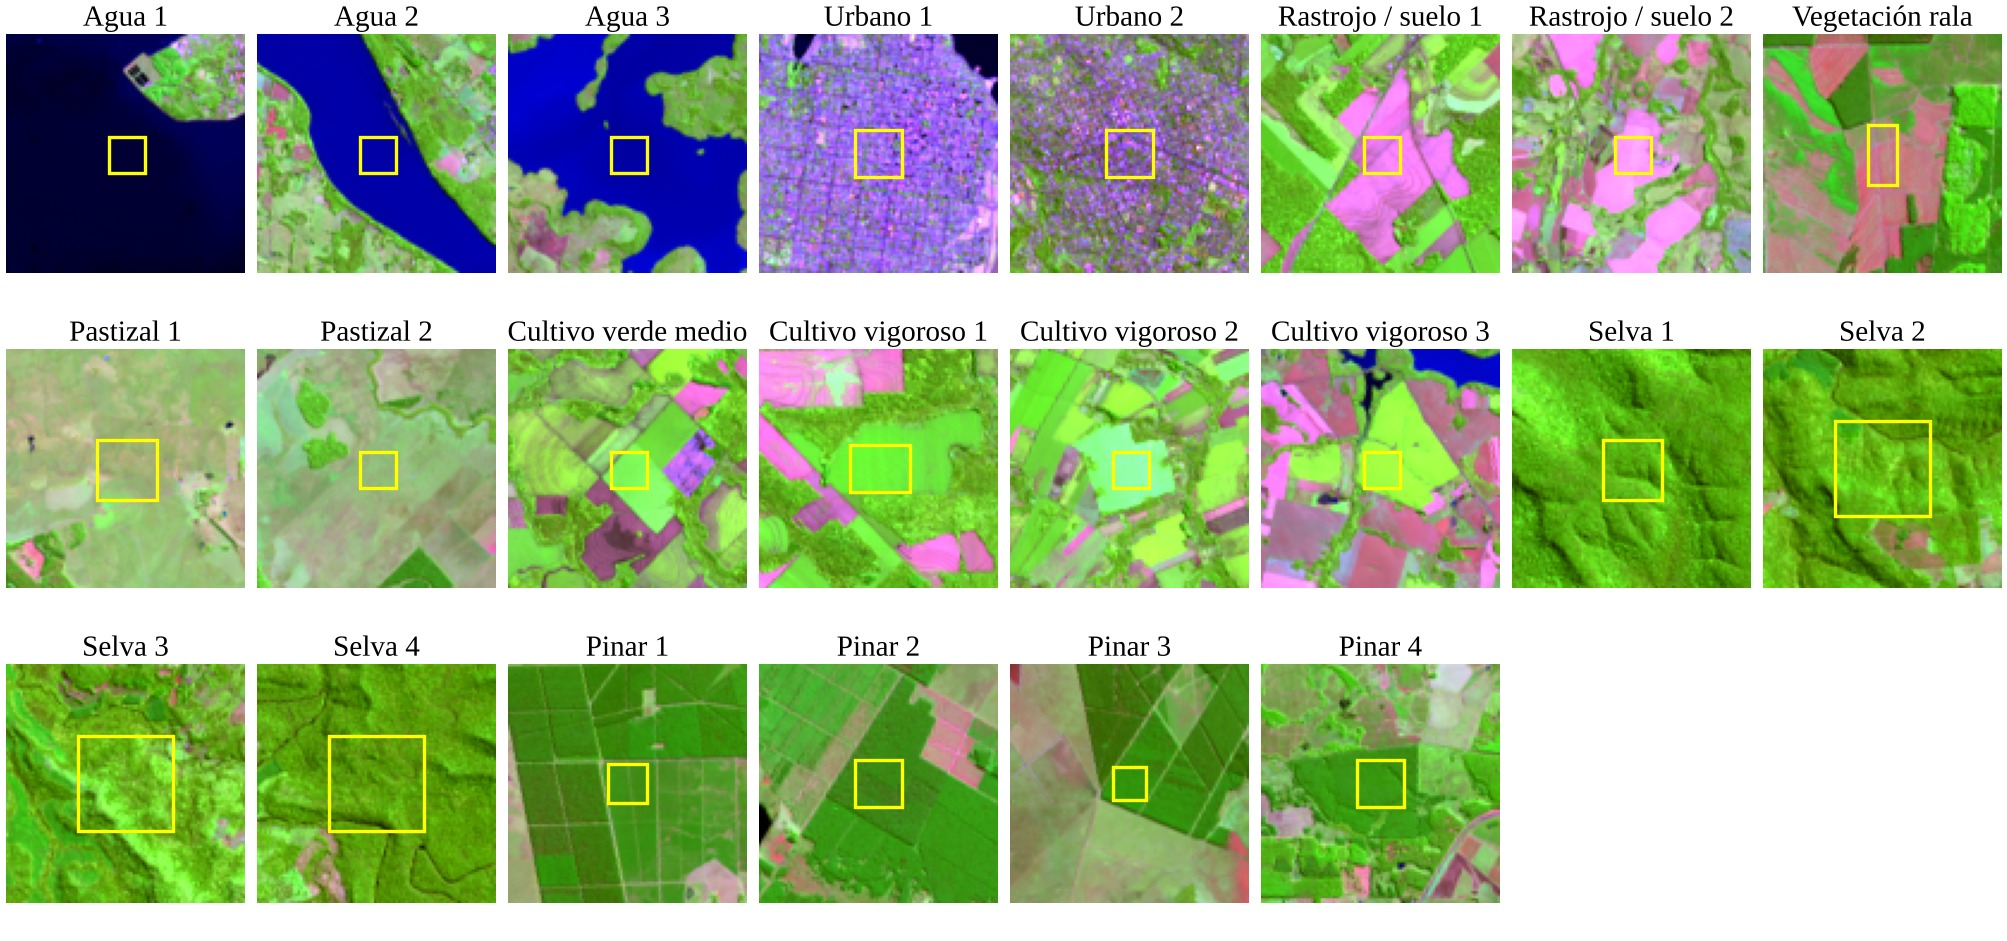
\includegraphics[width=\linewidth]{img/ejercicio3/muestras.jpg}
            \caption{Áreas de muestra (recuadro amarillo) con 3~km de entorno, en la composición 6-5-3.}
            \label{fig:ej3_muestras}
        \end{figure}

    \subsection{Bandas seleccionadas}

        La banda 5 mide el vigor, porque la estructura interna de la hoja refleja mucho el infrarrojo cercano. La banda 6 mide el agua de la hoja, que absorbe en esa región: la vegetación turgente es oscura y el suelo o el rastrojo, brillantes. La banda 3 corresponde al pico de reflectancia de la clorofila en el visible.

        Para comprobarlo se midió la firma espectral de cada cobertura (\textbf{Figura \ref{fig:ej3_firmas}}), es decir, la reflectancia de superficie media de sus píxeles de muestra en cada banda. Después se midió cuánto se separan dos coberturas con la separabilidad
        \[
            S = \frac{|\mu_1-\mu_2|}{\sigma_1+\sigma_2},
        \]
        donde $\mu$ y $\sigma$ son la media y el desvío estándar de la reflectancia de los píxeles de muestra de cada cobertura. El numerador es la distancia entre las dos coberturas y el denominador, la dispersión de cada una. Con $S = 1$ los rangos $\mu \pm \sigma$ de las dos apenas se tocan. Con $S > 1$ casi no se solapan, y con $S < 0{,}5$ se confunden. Es el índice de discriminación $M$ de Kaufman y Remer \cite{ej3_kaufman}, muy usado para elegir bandas, y es una versión simplificada de la razón de Fisher del ejercicio 2.

        $S$ mide una variable por vez, pero la composición y la clasificación usan las tres bandas juntas. Para medir la separación combinada se usó el discriminante lineal de Fisher \cite{ej3_richards}, que busca la combinación de bandas $w^\top x$ que más separa las dos coberturas, con $w = (\Sigma_1 + \Sigma_2)^{-1}(\mu_1 - \mu_2)$, donde $\Sigma$ es la covarianza de cada cobertura. Sobre esa combinación se calculó $S$. Como referencia se calculó también para el NDVI, $(B5-B4)/(B5+B4)$, el índice de vegetación más usado \cite{ej3_rouse}.

        \begin{figure}[H] \centering
            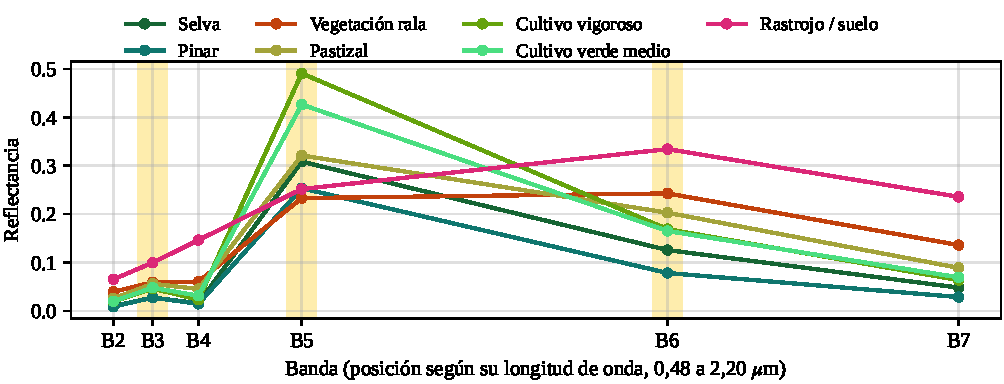
\includegraphics{img/ejercicio3/firmas.pdf}
            \caption{Firma espectral media de cada cobertura. Sombreadas, las bandas de la actividad.}
            \label{fig:ej3_firmas}
        \end{figure}

        \begin{table}[H] \centering
            \begin{tblr}{colspec = {lccccc}, row{1} = {font=\bfseries}}
                \toprule
                Par de coberturas & B3 & B5 & B6 & NDVI & B3, B5 y B6 \\
                \midrule
                Selva -- Pinar & 0,00 & 0,77 & \textbf{1,54} & 0,38 & 2,93 \\
                Selva -- Pastizal & 3,61 & 0,18 & 2,08 & \textbf{3,62} & 5,24 \\
                Selva -- Cultivo vigoroso & 0,98 & \textbf{1,54} & 0,82 & 0,39 & 2,08 \\
                Cultivo vigoroso -- Cultivo verde medio & 0,10 & 0,63 & 0,10 & \textbf{0,93} & 1,16 \\
                Pastizal -- Cultivo verde medio & 1,78 & \textbf{1,85} & 1,74 & 1,46 & 2,64 \\
                \bottomrule
            \end{tblr}
            \caption{Separabilidad $S$ entre pares de coberturas, calculada con sus píxeles de muestra, en cada banda, en el NDVI y en las tres bandas combinadas (discriminante de Fisher). En negrita, la mejor variable individual de cada par.}
            \label{tab:ej3_sep}
        \end{table}

        Ninguna banda separa sola todos los pares (\textbf{Tabla \ref{tab:ej3_sep}}). La 5 separa la selva del cultivo vigoroso, pero no del pastizal ($S = 0{,}18$), porque a fin del verano ambos reflejan entre 0,31 y 0,32 en el NIR. La banda 6 es la mejor para selva y pinar, y la 3 separa la selva del pastizal, pero no del pinar. Los estados de cultivo son el par más difícil: ninguna banda pasa de 0,63. Además, el NDVI se satura en la vegetación densa: la selva da 0,90 y el cultivo vigoroso 0,91. Combinadas, en cambio, las tres bandas separan todos los pares, con $S$ entre 1,16 y 5,24. Cada banda aporta algo distinto: la 5 la estructura del dosel, la 6 el contenido de agua y la 3 los tonos de verde. Por eso se usan las tres.

        La separabilidad depende de que las muestras representen toda la variación de cada cobertura. Con una sola área de selva y una de pinar, el NIR parecía separarlas ($S = 1{,}16$). Con cuatro áreas de cada una, en laderas al sol y en sombra y en plantaciones distintas, baja a 0,77.

    \subsection{Composición}

        Se compararon composiciones del anexo de la consigna midiendo la diferencia de color percibida entre las coberturas, con el color mediano de sus píxeles de muestra. Se usó la distancia $\Delta E$ en el espacio CIELAB, en el que distancias iguales se perciben como diferencias iguales y $\Delta E > 10$ es claramente otro color (\textbf{Tabla \ref{tab:ej3_de}} y \textbf{Figura \ref{fig:ej3_comp}}).

        \begin{table}[H] \centering
            \begin{tblr}{colspec = {lccc}, row{1} = {font=\bfseries}, row{7} = {font=\bfseries}}
                \toprule
                Composición (R-G-B) & $\Delta E$ medio & Cultivo vigoroso / medio & Selva / pinar \\
                \midrule
                4-3-2 color natural & 44,9 & 18,3 & 3,8 \\
                5-4-3 color infrarrojo & 62,4 & 14,7 & 13,1 \\
                6-5-2 agricultura & 77,7 & 2,5 & 13,9 \\
                6-5-4 análisis de vegetación & 76,5 & 3,1 & 14,1 \\
                5-6-3 & 55,7 & 14,1 & 19,2 \\
                6-5-3 (elegida) & 75,0 & 11,2 & 14,7 \\
                \bottomrule
            \end{tblr}
            \caption{Diferencia de color percibida $\Delta E$ entre las coberturas según la composición.}
            \label{tab:ej3_de}
        \end{table}

        \begin{figure}[H] \centering
            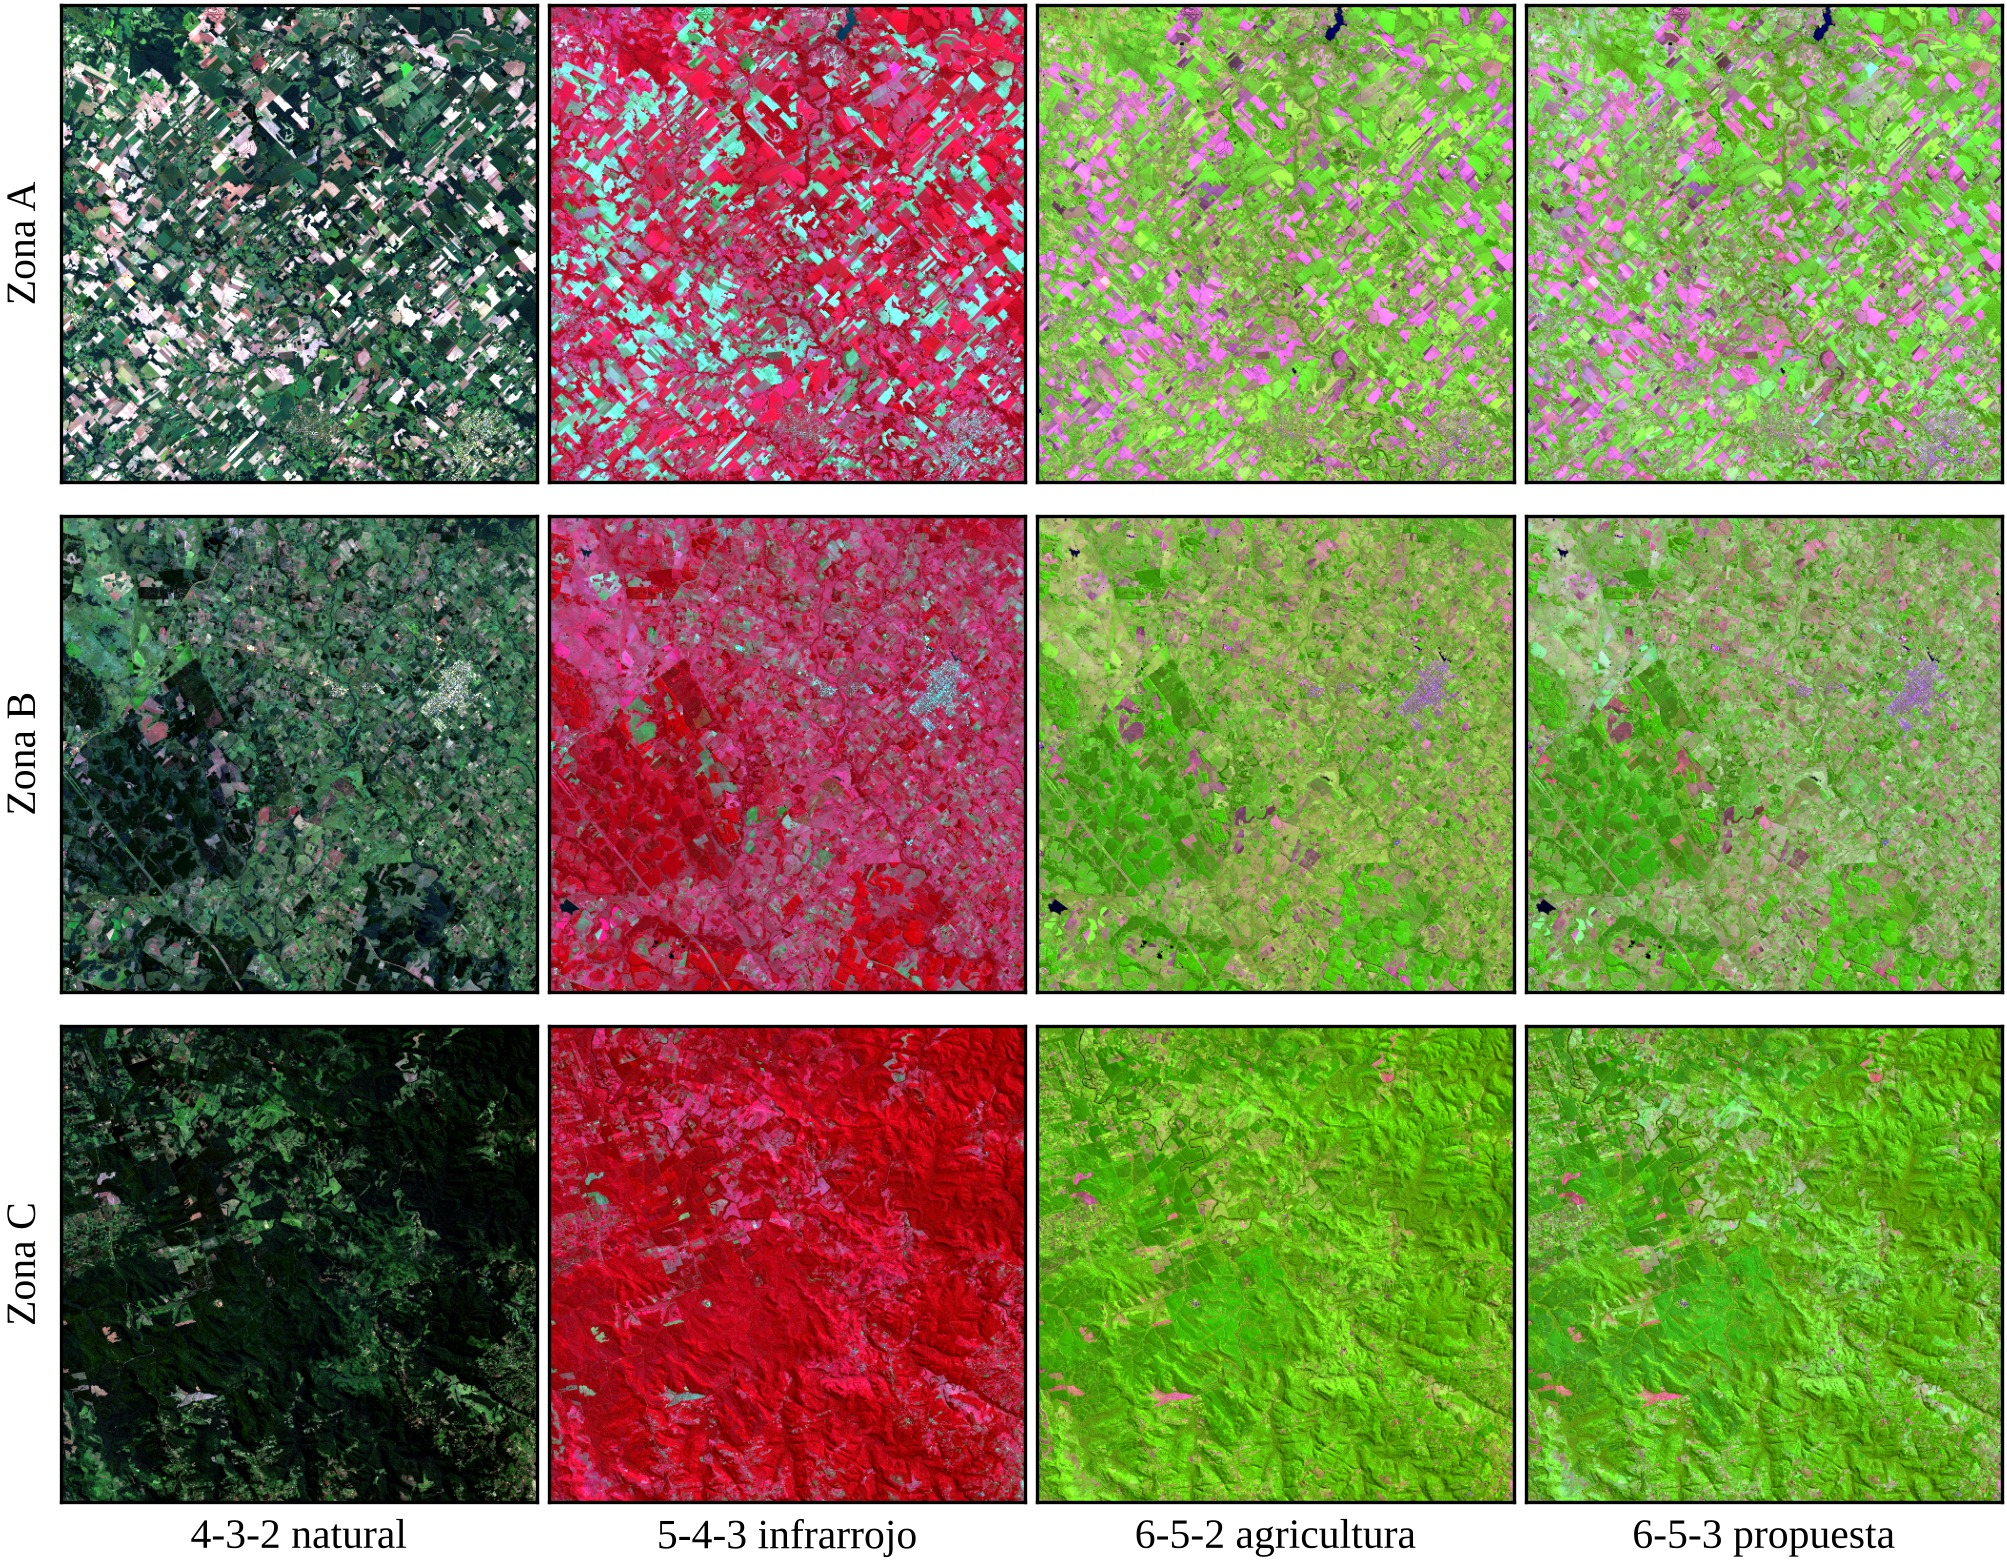
\includegraphics[width=.6\linewidth]{img/ejercicio3/composiciones.jpg}
            \caption{Zonas A, B y C (de arriba hacia abajo) con cuatro composiciones y el mismo estiramiento de contraste.}
            \label{fig:ej3_comp}
        \end{figure}

        En color natural la selva y el pinar son indistinguibles ($\Delta E = 3{,}8$) y en la zona C la selva se ve casi negra. Poner el NIR en el canal verde da el mayor contraste general y hace que la vegetación se vea verde. La banda del canal azul decide si se separan los estados de cultivo. Con la banda 3, el cultivo vigoroso y el verde medio quedan distintos ($\Delta E = 11{,}2$), mientras que con la 2 o la 4, como en las composiciones del anexo, quedan casi iguales. Entre las de mayor contraste ($\Delta E$ medio de 75 a 78), la 6-5-3 es la única que distingue los estados de cultivo.

        Se eligió la composición \textbf{6-5-3}: R~=~SWIR~1, G~=~NIR y B~=~verde. En ella el cultivo vigoroso y la selva en laderas al sol se ven verde brillante, la selva verde medio con textura, los pinares verde oscuro uniforme, el pastizal gris rosado, el rastrojo y el suelo magenta, la ciudad violeta y el agua azul oscuro. La selva en laderas en sombra también se ve oscura, pero con textura rugosa.

    \subsection{Mejora de contraste}

        Se compararon cuatro técnicas sobre la zona C (\textbf{Figura \ref{fig:ej3_realce}}). Sin realce la imagen queda oscura y aprovecha 5,4 bits de entropía. El estiramiento lineal entre los percentiles 2 y 98 calculados dentro de la zona amplía las pequeñas variaciones del SWIR~1 en el bosque, y la selva toma tonos pardos, como si estuviera seca. Con los mismos percentiles calculados sobre toda la escena la selva queda verde, con el mismo contraste (7,74 bits). La ecualización llega a la entropía máxima (8 bits), pero tiñe la selva de azul y magenta y los colores pierden su significado.

        \begin{figure}[H] \centering
            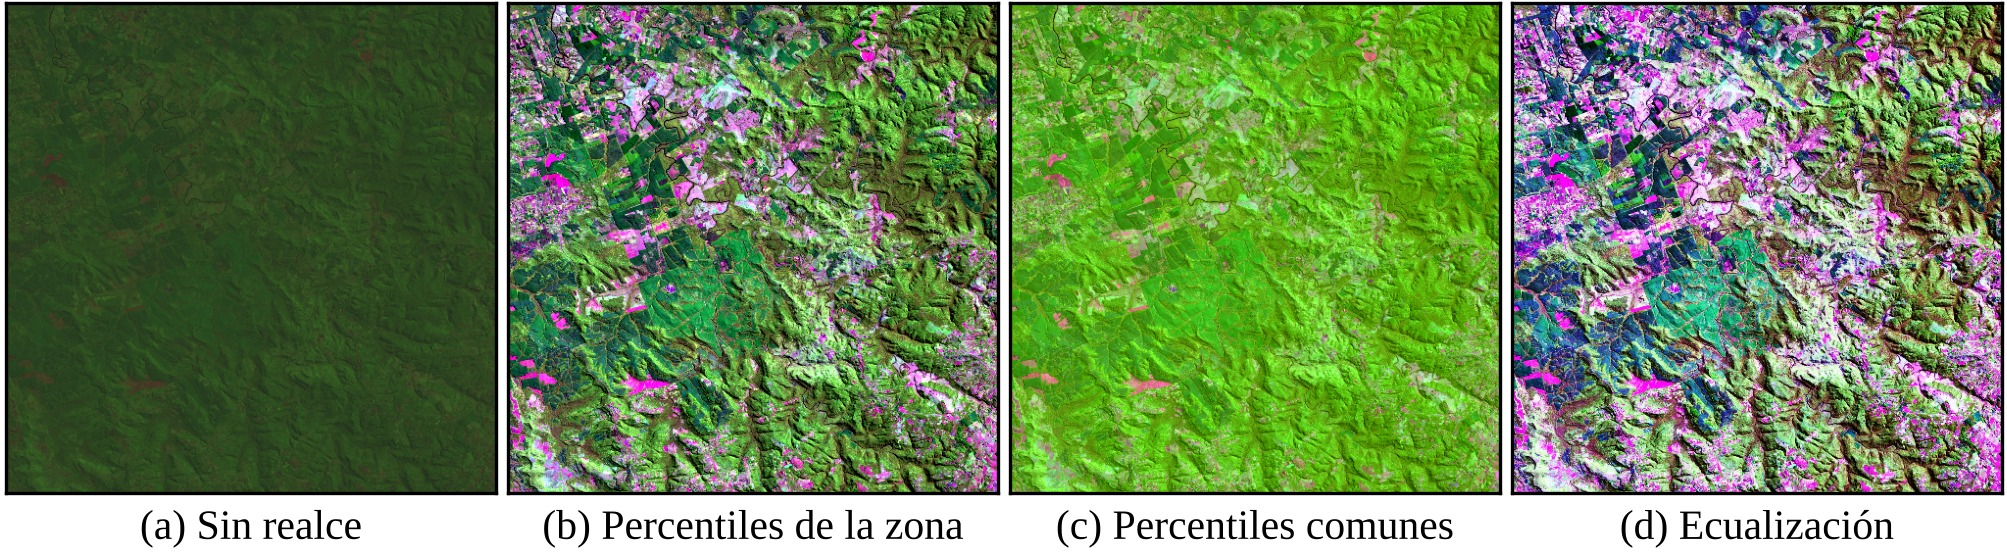
\includegraphics{img/ejercicio3/realce.jpg}
            \caption{Composición 6-5-3 de la zona C con distintas técnicas de realce.}
            \label{fig:ej3_realce}
        \end{figure}

        Se usó el estiramiento por percentiles comunes a toda la escena, para que un mismo color signifique lo mismo en cualquier zona. Los percentiles se calcularon solo con píxeles válidos. El relleno ocupa un tercio de la escena y, si se lo incluye como en el notebook de la cátedra, el percentil 2 da 0 en lugar de valores entre 7.400 y 8.100 cuentas según la banda.

    \subsection{Efecto del relieve}

        La zona C es casi toda selva sobre sierras. Para medir cómo cambia su firma con la iluminación se tomó el bosque de la sierra: unos 400.000 píxeles con NDVI~$> 0{,}85$, sin el cuadrante noroeste de la zona, que tiene chacras y plantaciones, y sin las áreas de muestra. Se compararon las laderas en sombra y al sol, es decir el 15\,\% de los píxeles con menor y mayor NIR. Dentro del mismo bosque el NIR va de 0,21 a 0,40, casi el doble.

        La selva en sombra, con un NIR de 0,22 y una banda 6 de 0,09, se parece al pinar. En la composición 6-5-3 queda a $\Delta E = 11{,}4$ de su color, apenas por encima del umbral de 10, y la separabilidad en las bandas 5 y 6 es de solo 0,80 y 0,31. Combinando las tres bandas, en cambio, $S = 2{,}13$: la diferencia está en la proporción entre bandas, porque el pinar tiene menos SWIR~1 en relación con el NIR. La selva al sol se parece más al cultivo vigoroso ($\Delta E = 13{,}2$) que al color típico de la selva ($\Delta E = 21{,}7$), y combinando las tres bandas se separa poco de él ($S = 1{,}28$).

        Las proporciones entre las bandas 3, 5 y 6 son las mismas en sombra y al sol (0,063 : 0,673 : 0,263 y 0,062 : 0,676 : 0,262), porque la ladera multiplica las tres bandas por casi el mismo factor. Por eso los cocientes entre bandas no cambian con la iluminación.

    \subsection{Agrupamiento de las zonas}

        Para comprobar que la separación no depende solo del color, se agruparon los píxeles con k-medias, que forma $k$ grupos de píxeles con valores parecidos sin información previa sobre qué es cada cosa. Se hizo una sola vez para las tres zonas juntas, así cada grupo significa lo mismo en todas, y tanto las variables como el número de grupos se eligieron midiendo.

        \textbf{Variables.} Con las reflectancias, desde $k = 3$ la selva en sombra y la selva al sol caen siempre en grupos distintos. K-medias no conoce la variación de cada cobertura, y la mayor diferencia entre píxeles es el brillo, que en la sierra depende de la ladera, así que el agrupamiento separa laderas en lugar de coberturas. Por eso se agrupó con dos cocientes que usan solo las bandas del ejercicio y no cambian con la iluminación: el GNDVI, $(B5-B3)/(B5+B3)$, y el NDMI, $(B5-B6)/(B5+B6)$, que mide el agua de la vegetación \cite{ej3_gao}. Con ellos, entre el 92 y el 100\,\% de la selva en sombra y al sol cae en los mismos grupos para cualquier $k$. El agua se separó antes por regla (NIR~$< 0{,}05$).

        \textbf{Número de grupos.} Se probó $k$ de 2 a 8 con dos medidas. La inercia es la distancia cuadrática media de cada píxel al centro de su grupo: baja un 57\,\% de $k = 2$ a 3 y después cada vez menos (33, 29 y 24\,\%). La silueta compara, para cada píxel, la distancia media a su grupo con la del grupo más cercano, y vale 1 cuando los grupos están bien separados. Se mantiene en 0,60 y 0,58 hasta $k = 3$ y cae a 0,50 con $k = 4$. Con las reflectancias, en cambio, no pasa de 0,38 para ningún $k$. Se eligió $k = 3$, porque con $k = 2$ solo se separa la vegetación densa del resto y con más grupos se parte en pedazos una nube continua de valores.

        \begin{figure}[H] \centering
            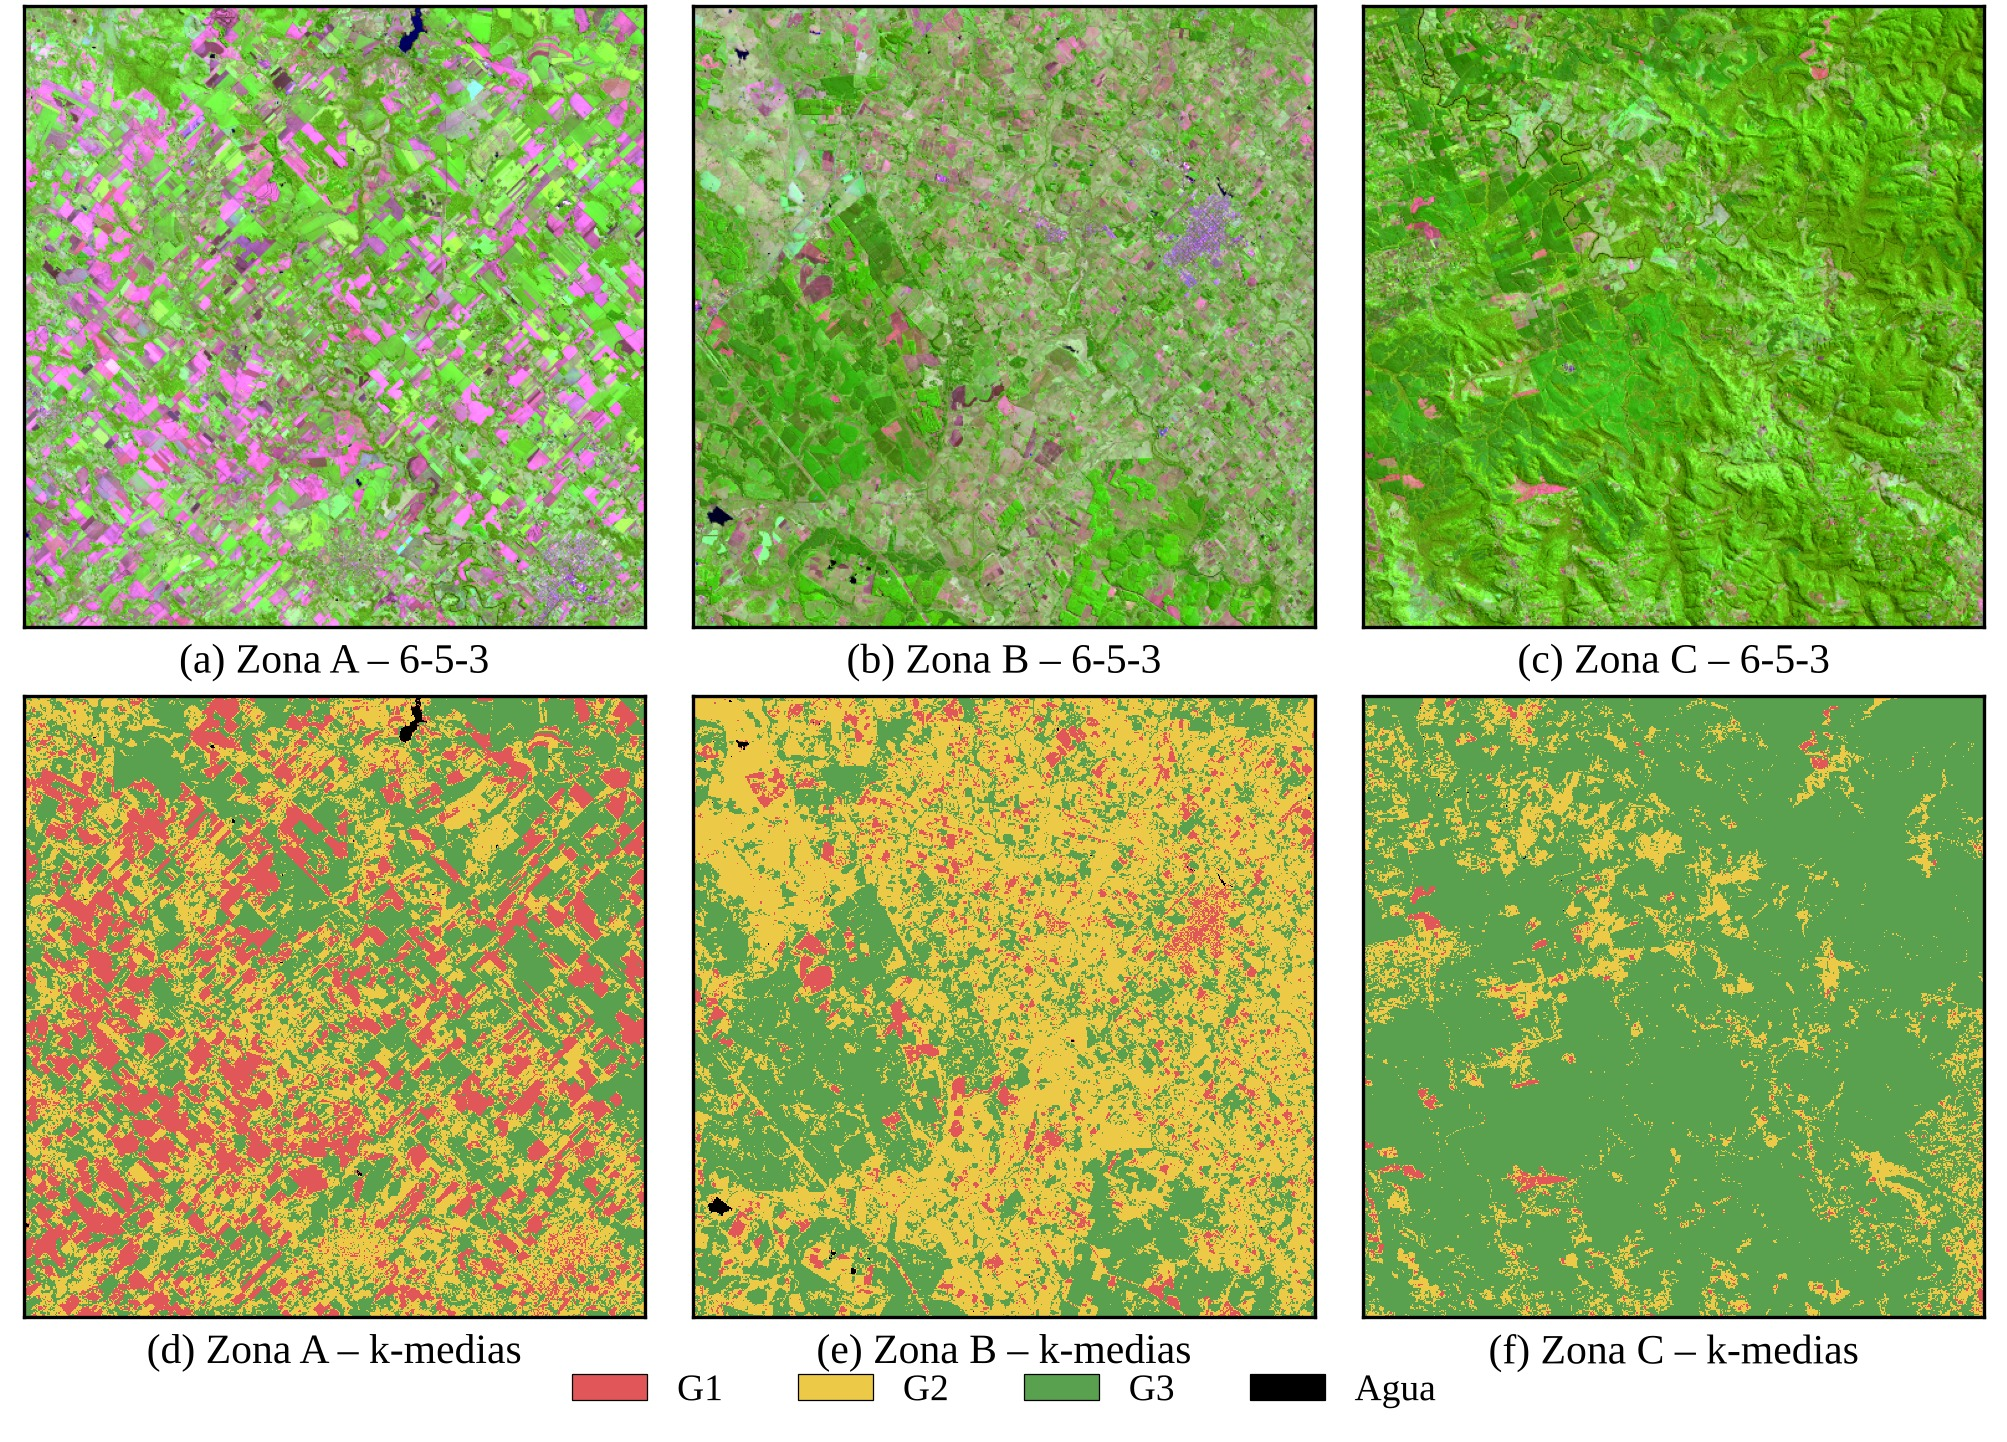
\includegraphics[width=.66\linewidth]{img/ejercicio3/kmedias.jpg}
            \caption{Composición 6-5-3 (arriba) y grupos de k-medias con el GNDVI y el NDMI, calculados para las tres zonas juntas (abajo).}
            \label{fig:ej3_kmedias}
        \end{figure}

        \begin{table}[tbp] \centering \footnotesize
            \begin{tblr}{colspec = {cX[l]ccc}, width = \linewidth, row{1} = {font=\bfseries}, rowsep = 2pt, stretch = 1}
                \toprule
                Grupo & Interpretación & Zona A & Zona B & Zona C \\
                \midrule
                \grupo{E15759}{G1} & Suelo desnudo, rastrojo y ciudad & 25\,\% & 7\,\% & 1\,\% \\
                \grupo{EDC948}{G2} & Vegetación intermedia: pastizal, cultivo en desarrollo o maduro, claros & 34\,\% & 56\,\% & 15\,\% \\
                \grupo{59A14F}{G3} & Vegetación densa y saludable: selva, monte, forestación y cultivo vigoroso & 41\,\% & 36\,\% & 84\,\% \\
                \bottomrule
            \end{tblr}
            \caption{Interpretación de los grupos de k-medias y porcentaje del área de cada zona.}
            \label{tab:ej3_km}
        \end{table}

        En la zona A el ciclo agrícola se reparte en los tres grupos, con lotes enteros de un mismo grupo (\textbf{Figura \ref{fig:ej3_kmedias}d}), y en la zona B domina el pastizal. En la zona C el 84\,\% es vegetación densa, y en ese grupo están el 98\,\% de la selva en sombra y el 100\,\% de la selva al sol. El G2 de la zona C corresponde a los claros y chacras del noroeste y a algunos claros dentro de la sierra. La separación entre suelo, vegetación intermedia y vegetación densa está en los datos y no solo en el color. Dentro de G3, selva, pinar y cultivo vigoroso tienen cocientes cercanos (GNDVI de 0,80 a 0,84 y NDMI de 0,42 a 0,53) comparados con la distancia entre grupos, y no forman grupos propios. Para separarlos hacen falta muestras de cada clase.

    \subsection{Clasificación supervisada}

        Para ubicar los objetivos en toda la escena se hizo una clasificación supervisada de máxima verosimilitud con las bandas 3, 5 y 6, entrenada con las áreas de muestra \cite{ej3_richards}. De cada clase se calcula su firma media y su covarianza, y cada píxel se asigna a la clase más probable según la distancia de Mahalanobis, que tiene en cuenta las tres bandas juntas y cómo varían dentro de cada clase. Si está demasiado lejos de todas, queda sin clasificar. El agua se asigna por regla (NIR~$< 0{,}05$), y al final un filtro de mayoría de $3 \times 3$ elimina los píxeles sueltos. Se probaron dos mejoras pensadas para el efecto del relieve:

        \begin{itemize}
            \item \textbf{Subclases de selva.} Una sola clase con toda la variación de iluminación queda muy ancha. La selva en sombra cae en un extremo de su distribución, y el pinar, más compacto, resulta más probable. Por eso la selva se dividió en tres subclases según el brillo (tercios del NIR de sus muestras), que al final se unen.
            \item \textbf{Textura.} Una plantación es pareja, mientras que la selva sobre relieve alterna laderas al sol y en sombra en pocas decenas de metros. Se midió con el coeficiente de variación local del NIR, $\sigma_{\text{local}} / \mu_{\text{local}}$, en una ventana de $9 \times 9$ píxeles (270~m), calculado con dos filtros de promedio, de la imagen y de su cuadrado (\textbf{Figura \ref{fig:ej3_textura}b}). El pinar da $0{,}041 \pm 0{,}020$ en sus áreas de muestra y la selva en sombra $0{,}170 \pm 0{,}055$ ($S = 1{,}72$). Sumada a las tres bandas, la separabilidad entre ambas sube de 2,13 a 2,55. Se usó solo para decidir entre pinar y selva: un píxel clasificado como pinar pasa a selva si su textura supera la media más dos desvíos del pinar. Como la textura depende del entorno, y en una plantación real el entorno incluye cortafuegos y bordes, el umbral se calculó con bloques de $60 \times 60$ píxeles alrededor de cada plantación (0,136). Con el interior de los compartimentos (0,080) se marcaría el 97\,\% de la selva en sombra, pero se borraría el 29\,\% del pinar de los bloques.
        \end{itemize}

        Las tres variantes se evaluaron en 16 áreas de validación que no se usaron para entrenar, en los bloques completos de las plantaciones de validación y en el bosque de la sierra (\textbf{Tabla \ref{tab:ej3_val}} y \textbf{Figura \ref{fig:ej3_textura}}).

        \begin{figure}[H] \centering
            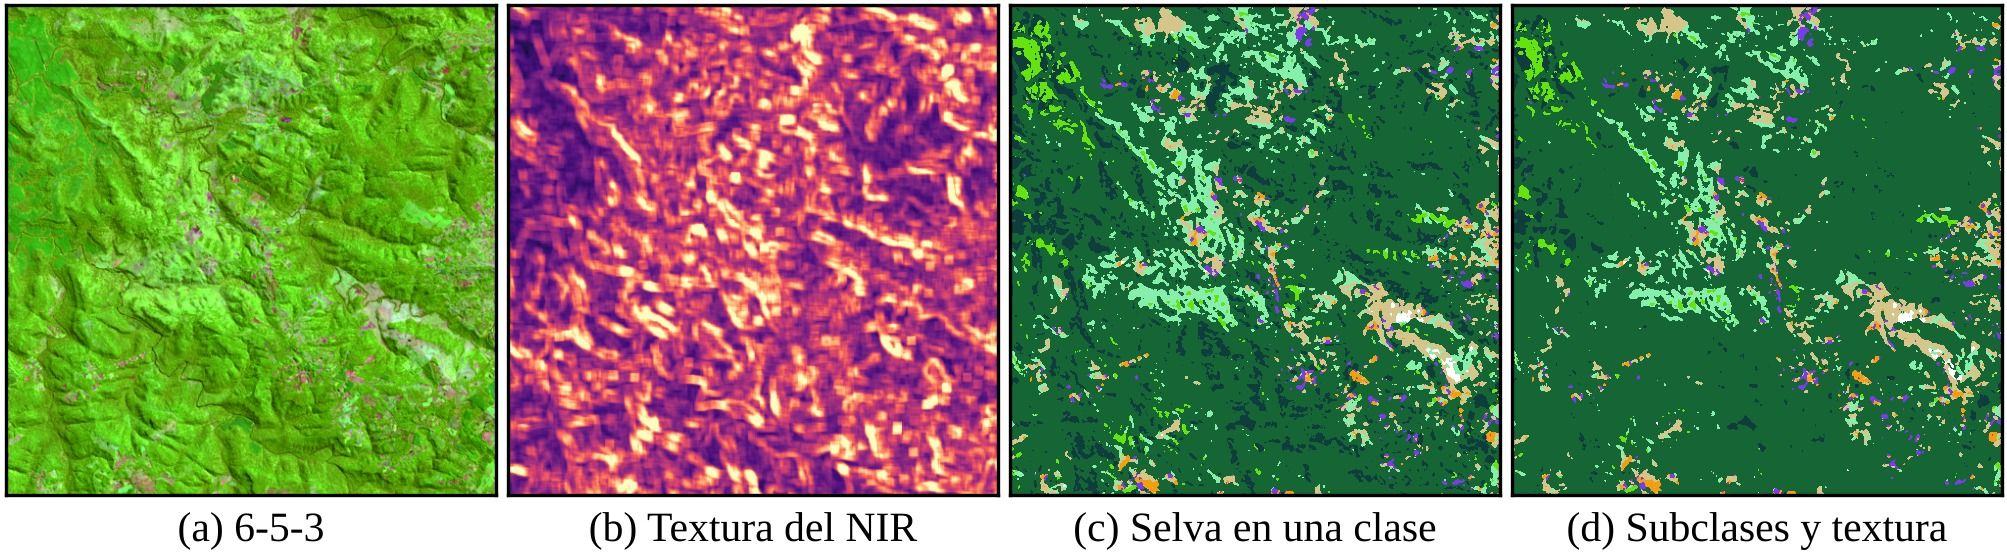
\includegraphics{img/ejercicio3/textura.jpg}
            \caption{Sector de 15~km de la zona C: composición 6-5-3, textura del NIR (más clara, más rugosa) y clasificación supervisada con la selva en una clase y con subclases y textura. En verde oscuro, la selva; en verde petróleo, el pinar; en verde claro, el cultivo verde medio.}
            \label{fig:ej3_textura}
        \end{figure}

        \begin{table}[H] \centering
            \begin{tblr}{colspec = {lccc}, row{1} = {font=\bfseries}}
                \toprule
                Píxeles clasificados correctamente & Selva en una clase & Subclases & Subclases y textura \\
                \midrule
                Selva con relieve (validación) & 82\,\% & 92\,\% & 95\,\% \\
                Selva en sombra de la sierra & 58\,\% & 85\,\% & 93\,\% \\
                Selva al sol de la sierra & 52\,\% & 71\,\% & 71\,\% \\
                Áreas de pinar (validación) & 99 a 100\,\% & 99 a 100\,\% & 99 a 100\,\% \\
                Bloques de pinar completos & 96\,\% & 93\,\% & 92\,\% \\
                Promedio de las 16 áreas & 98\,\% & 99\,\% & 99\,\% \\
                \bottomrule
            \end{tblr}
            \caption{Acierto de la clasificación supervisada según cómo se modela la selva.}
            \label{tab:ej3_val}
        \end{table}

        Con la selva en una sola clase, el 42\,\% de la selva en sombra se clasificaba como pinar. Con subclases baja al 15\,\%, y con la textura al 7\,\%. Es decir, el problema no eran las bandas, que separan la selva en sombra del pinar, sino cómo se modelaba la selva. Las mejoras le cuestan poco al pinar: en los bloques completos, con cortafuegos y bordes cerca, se clasifica como pinar entre el 92 y el 96\,\%. La selva al sol sube de 52 a 71\,\%, pero el 28\,\% sigue como cultivo, sobre todo cultivo verde medio. La textura no ayuda ahí, porque las laderas al sol también son rugosas (0,13). El acierto promedio queda entre 98 y 99\,\% en las tres variantes, porque las mejoras solo cambian las áreas afectadas por el relieve.

        \begin{figure}[H] \centering
            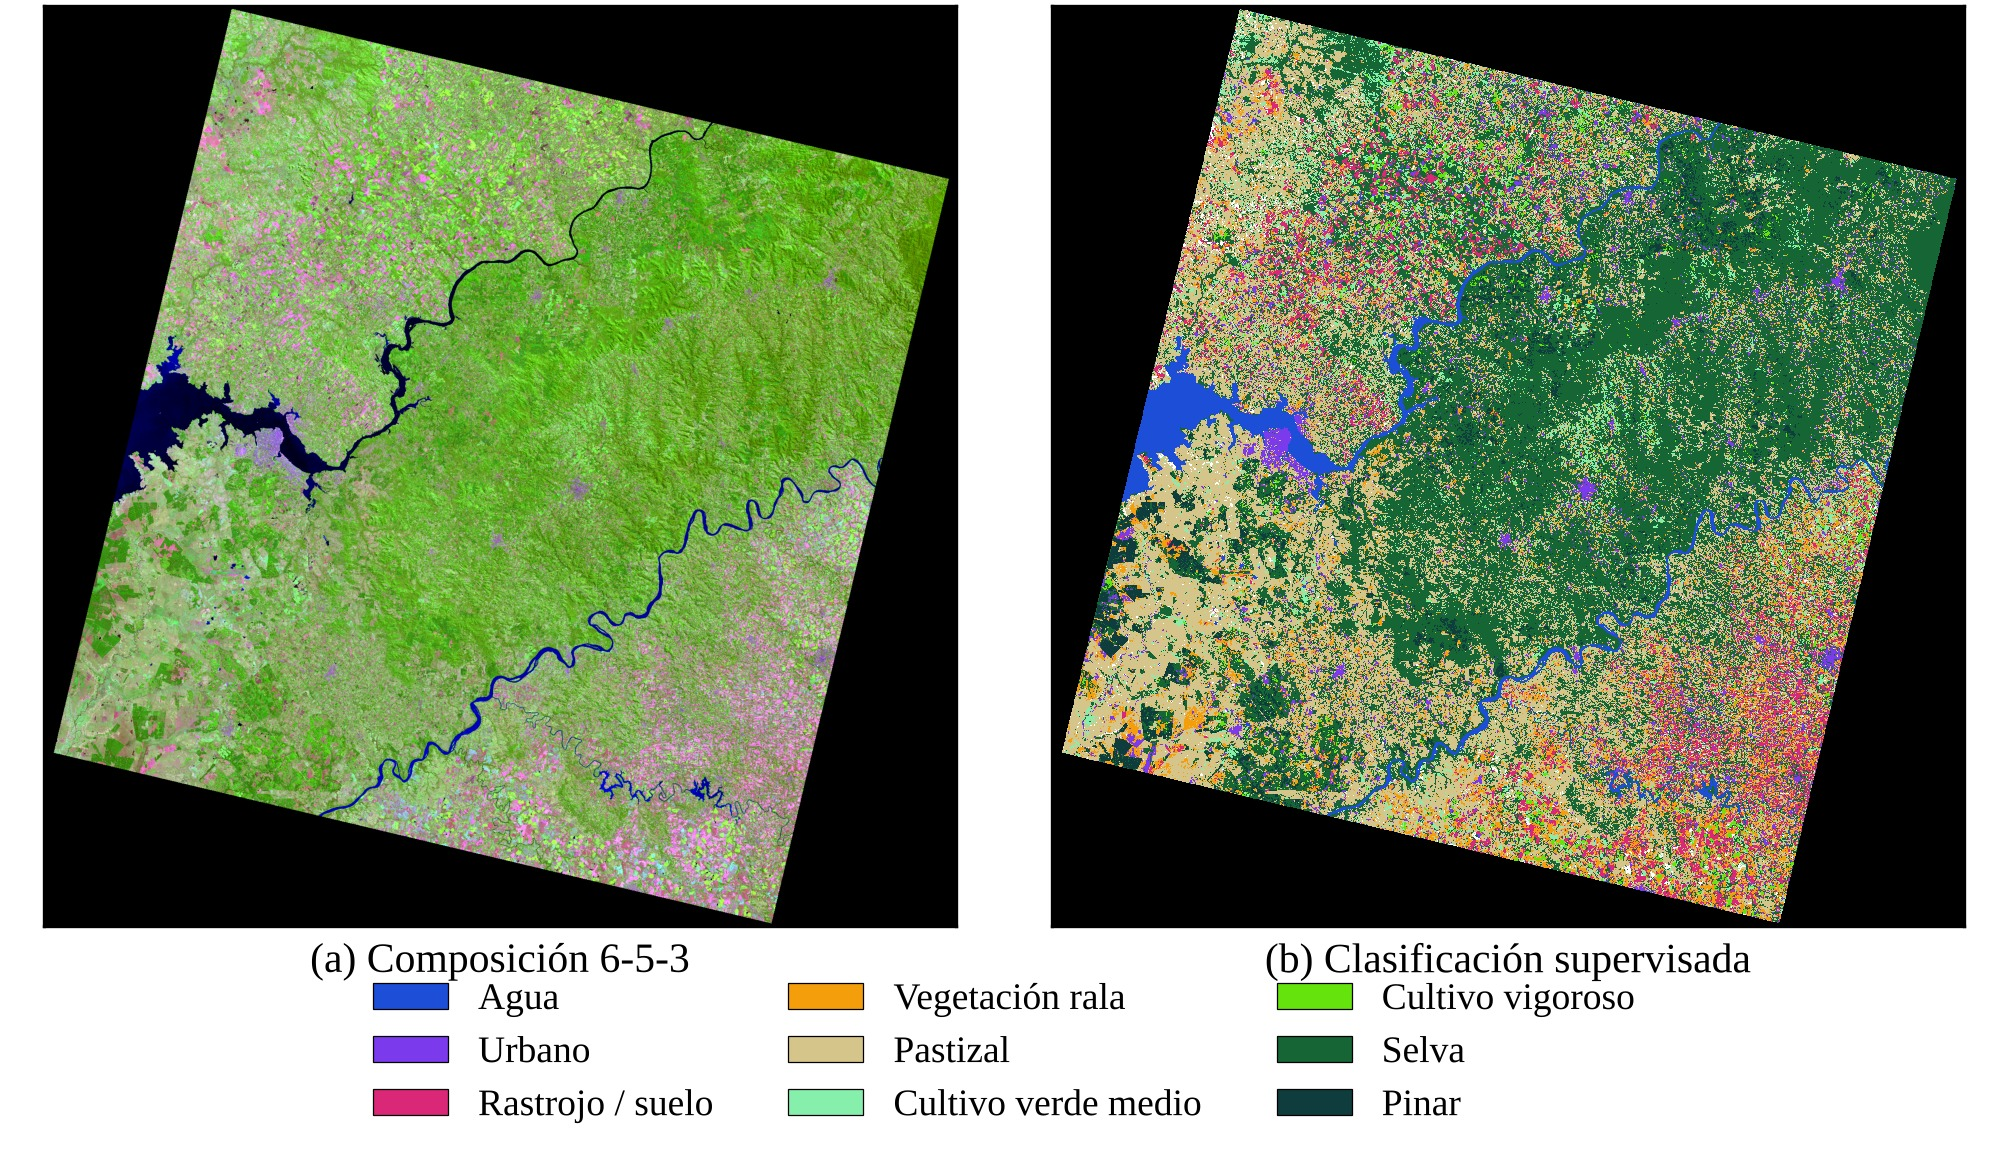
\includegraphics[width=.72\linewidth]{img/ejercicio3/clasificacion.jpg}
            \caption{Escena completa en la composición 6-5-3 y clasificación supervisada con subclases de selva y textura.}
            \label{fig:ej3_clasif}
        \end{figure}

        En la \textbf{Figura \ref{fig:ej3_clasif}} la vegetación densa y saludable forma un bloque continuo sobre la Sierra Central, con unos 16.100~km$^2$ de selva y monte. Las forestaciones de pino suman unos 1.050~km$^2$, sobre todo en Corrientes, y el cultivo vigoroso unos 510~km$^2$. Los cultivos se concentran en Itapúa y en el noroeste de Rio Grande do Sul, donde predominan el rastrojo y la vegetación rala porque la cosecha estaba más avanzada. Quedan dos errores visibles: parte de la selva en laderas al sol figura como cultivo verde medio, y la clase urbana, con 1.640~km$^2$, aparece también en píxeles sueltos de las zonas agrícolas del sureste, donde no hay ciudades.

    \subsection{Conclusiones}

        La composición 6-5-3 con estiramiento por percentiles de toda la escena resalta la vegetación densa y saludable y separa monte, forestaciones, pastizal y estados de cultivo que en color natural se confunden. Ninguna de las tres bandas separa sola todas las coberturas, pero combinadas separan todos los pares estudiados.

        La principal dificultad es el relieve, que cambia la firma de la selva según la ladera, y las mediciones solo lo muestran si las muestras cubren esa variación y son puras: áreas con cortafuegos o con dos campos distintos falseaban la textura y la validación. Los cocientes de bandas lo eliminan en el agrupamiento. En la clasificación, las subclases de iluminación y la textura recuperan la selva en sombra (93\,\%), pero la selva al sol se sigue confundiendo en parte con el cultivo (71\,\%). Es el límite de estas bandas en una sola fecha; corregirlo requeriría un modelo de elevación del terreno.

        La resolución de 30~m alcanza para lotes mecanizados y bloques forestales, no para chacras chicas, hileras de yerba o té ni árboles aislados. Para saber qué especie se cultiva harían falta varias fechas, datos de campo o más resolución.
